% !TeX program = lualatex
% From figures/: run `latexmk -lualatex -interaction=nonstopmode -halt-on-error -output-directory=generated tree_approximation_ratio_2d_plot.tex`.
% The manuscript includes the resulting cached PDF instead of recalculating
% this PGFPlots diagram during every compilation.
\documentclass[11pt,border=2pt]{standalone}
\usepackage{tikz}
\usepackage{pgfplots}
\usepackage{amsmath}
\pgfplotsset{compat=1.18}
% Define colors
\definecolor{cutA}{RGB}{214,39,40}
\definecolor{cutB}{RGB}{31,119,180}
\definecolor{cutC}{RGB}{44,160,44}
\definecolor{cutD}{RGB}{23,190,207}
\definecolor{cutE}{RGB}{148,103,189}
\definecolor{cutF}{RGB}{140,86,75}

% Bracket and notation macros
\newcommand{\br}[1]{\mathopen{}\left( #1 \right)}
\newcommand{\brc}[1]{\mathopen{}\left\{ #1 \right\}}
\newcommand{\spr}[1]{\mathopen{}\left| #1 \right|}
\newcommand{\fl}[1]{\mathopen{}\left\lfloor #1 \right\rfloor}
\newcommand{\cl}[1]{\mathopen{}\left\lceil #1 \right\rceil}
\newcommand{\angl}[1]{\mathopen{}\langle #1 \rangle}
\newcommand{\e}[1]{\exp\left\{ #1 \right\}}

% Algorithm and notation
\newcommand{\Cent}{\texttt{Cent}}
\newcommand{\APP}{\texttt{APP}}
\newcommand{\DPartition}{\textsc{DPartition}}
\newcommand{\cut}{\delta}
\newcommand{\Etree}{\mathbb{E}_{T\sim\mu}}
\newcommand{\DD}[1]{\textcolor{red}{DD: #1}}
\newcommand{\DDfix}[1]{\textcolor{violet}{#1}}
\newcommand{\bigo}{\mathcal{O}}
\newcommand{\minCut}[3]{\textup{min-cut}_{#3}\br{#1,#2}}
\newcommand{\phiwK}{\phi_w^{K}}
\newcommand{\OPTh}{\OPT_h^{\delta}}
\newcommand{\OPTc}{\OPT_{\psi}}
\newcommand{\OPTdem}[2]{\OPT_{#2}\br{#1}}
\newcommand{\paths}{P^*}
\newcommand{\OPT}{\textup{OPT}}
\DeclareMathOperator*{\argmin}{arg\,min}
\DeclareMathOperator*{\argmax}{arg\,max}
\newcommand{\cov}{\text{cov}}
\newcommand{\ct}{\text{ct}}
\newcommand{\Sopt}{S_h^{*}}
\newcommand{\SoptBar}{\bar{S}_h^{*}}
\newcommand{\hw}{h_w^{\delta}}
\newcommand{\hOPT}{S_h^{\delta}(G)}
\newcommand{\psiOPT}{S_{\psi}(G)}
\newcommand{\COST}{{c}}
\newcommand{\dist}{\text{dist}}
\newcommand{\ch}{\text{ch}}
\newcommand{\supp}{\operatorname{supp}}
\newcommand{\vol}{\operatorname{vol}}
\newcommand{\lca}{\operatorname{lca}}

% Calligraphic letter macros
\newcommand{\cA}{\mathcal{A}}
\newcommand{\cB}{\mathcal{B}}
\newcommand{\cC}{\mathcal{C}}
\newcommand{\cD}{\mathcal{D}}
\newcommand{\cE}{\mathcal{E}}
\newcommand{\cF}{\mathcal{F}}
\newcommand{\cG}{\mathcal{G}}
\newcommand{\cH}{\mathcal{H}}
\newcommand{\cI}{\mathcal{I}}
\newcommand{\cJ}{\mathcal{J}}
\newcommand{\cK}{\mathcal{K}}
\newcommand{\cL}{\mathcal{L}}
\newcommand{\cM}{\mathcal{M}}
\newcommand{\cN}{\mathcal{N}}
\newcommand{\cO}{\mathcal{O}}
\newcommand{\cP}{\mathcal{P}}
\newcommand{\cQ}{\mathcal{Q}}
\newcommand{\cR}{\mathcal{R}}
\newcommand{\cS}{\mathcal{S}}
\newcommand{\cT}{\mathcal{T}}
\newcommand{\cU}{\mathcal{U}}
\newcommand{\cV}{\mathcal{V}}
\newcommand{\cW}{\mathcal{W}}
\newcommand{\cX}{\mathcal{X}}
\newcommand{\cY}{\mathcal{Y}}
\newcommand{\cZ}{\mathcal{Z}}

\begin{document}
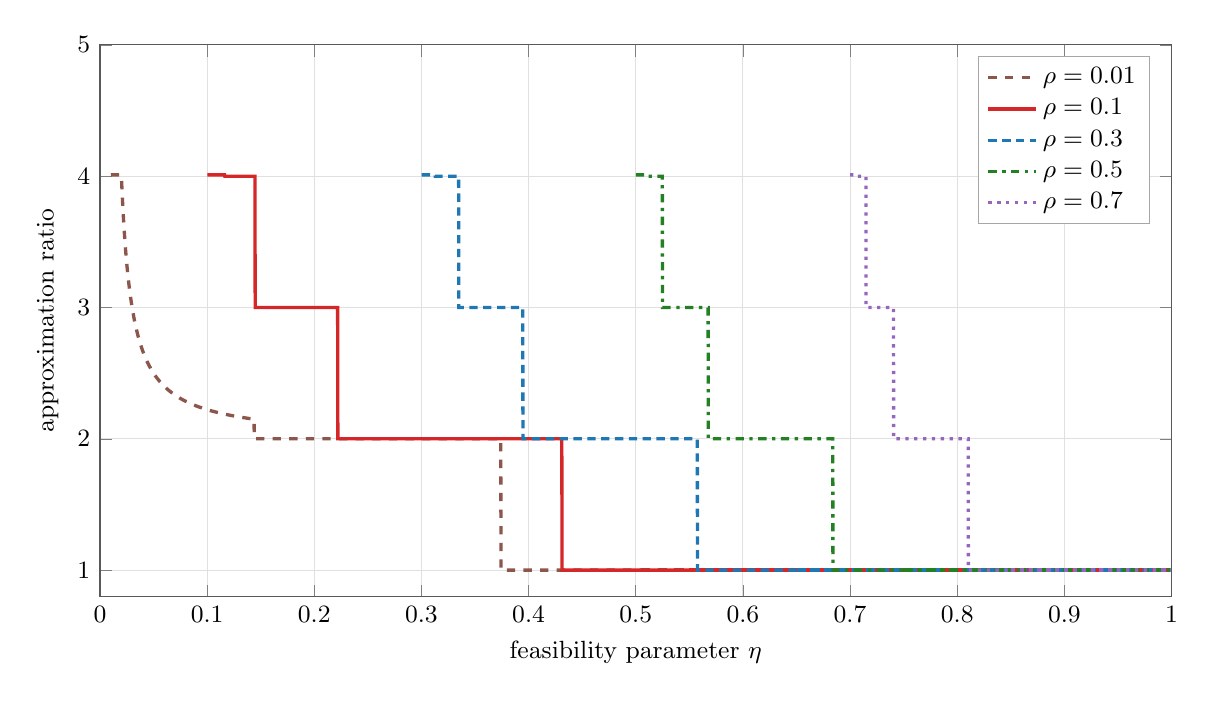
\begin{tikzpicture}
  \begin{axis}[
    width=15.19cm,
    height=8.585cm,
    xmin=0,
    xmax=1,
    ymin=0.8,
    ymax=5,
    xlabel={feasibility parameter $\eta$},
    ylabel={approximation ratio},
    xtick={0,0.1,...,1},
    ytick={1,2,3,4,5},
    grid=major,
    grid style={draw=black!12},
    axis line style={draw=black!65},
    tick label style={font=\small},
    label style={font=\small},
    legend style={
      font=\small,
      at={(0.98,0.98)},
      anchor=north east,
      draw=black!35,
      fill=white,
      cells={anchor=west}
    },
    samples=2000,
    no marks,
    unbounded coords=jump,
    restrict y to domain=0.8:5
  ]
    \addplot[draw=cutF,very thick,dashed,domain=0.010053:0.505]
      {min(5,min(4.01,min(2*x/(x-0.01),ceil(ln((1-0.01)/(x-0.01)))))};
    \addlegendentry{$\rho=0.01$}
    \addplot[draw=cutF,very thick,dashed,domain=0.5051:0.999,forget plot] {1};

    \addplot[draw=cutA,very thick,domain=0.1003:0.55]
      {min(5,min(4.01,min(2*x/(x-0.1),ceil(ln((1-0.1)/(x-0.1)))))};
    \addlegendentry{$\rho=0.1$}
    \addplot[draw=cutA,very thick,domain=0.5501:0.999,forget plot] {1};

    \addplot[draw=cutB,very thick,densely dashed,domain=0.30025:0.65]
      {min(5,min(4.01,min(2*x/(x-0.3),ceil(ln((1-0.3)/(x-0.3)))))};
    \addlegendentry{$\rho=0.3$}
    \addplot[draw=cutB,very thick,densely dashed,domain=0.6501:0.999,forget plot] {1};

    \addplot[draw=cutC!80!black,very thick,dashdotted,domain=0.50018:0.75]
      {min(5,min(4.01,min(2*x/(x-0.5),ceil(ln((1-0.5)/(x-0.5))))))};
    \addlegendentry{$\rho=0.5$}
    \addplot[draw=cutC!80!black,very thick,dashdotted,domain=0.7501:0.999,forget plot] {1};

    \addplot[draw=cutE,very thick,dotted,domain=0.7001:0.85]
      {min(5,min(4.01,min(2*x/(x-0.7),ceil(ln((1-0.7)/(x-0.7))))))};
    \addlegendentry{$\rho=0.7$}
    \addplot[draw=cutE,very thick,dotted,domain=0.8501:0.999,forget plot] {1};
  \end{axis}
\end{tikzpicture}
\end{document}